\epigraph{\emph{
  ``Coming up with features is difficult, time-consuming, requires expert knowledge. "Applied machine learning" is basically feature engineering.''
}}{ Andrew Ng }

Considering the ``right'' features for clustering is a demanding and error prone process. Currently there is really just one way of describing documents: The vector space model. It breaks down to counting occurences and cooccurences of words and measuring distance by mathematical functions. We could just take all the words of a document, removing stopwords, and put them into a feature vector. This results in dimensionality explosion and extreme noise. Contrary to a document vector $d = \{w_1,w_2..w_n\}$, the feature vector represents a document by concepts $\{c_1,c_2,..c_j\}$. It is a projection of the original document often by fewer dimensions and a lifting of words. This lifting is bestly described as combining several words of a document, often occuring in the same sentence, extracting a shared meaning. We hope to find fewer words that share enough information with the original word, that the following holds:
  
  \begin{equation}
    f : d=\{w_1,w_2,..w_n\} \to \{c_1,c_2,..c_j\}
  \end{equation}

The function $f$ transforms a sequence of words $w_1..w_n$ of a document $d$ to a sequence of concepts $c_1..c_j$. The concepts can be derived in a lot of ways.

  \begin{enumerate}
    \item Pruning words of low and high significance.
    \item Using syntactic parsing to retrieve noun phrases, named entity tags or part of speech tags.
    \item Using ontologies of wordnet to derive a shared meaning of words.
    \item Mapping documents to wikipedia categories.
    \item Using kernel methods, preselecting initial clusters in a semi-supervised way.
  \end{enumerate}

In the end, feature selection is probably the most demanding task. Expert knolwedge needs to be applied and can change over time. A computer handles documents in vector space, by counting. A human however perceives content differently. For any sufficiently adavanced algorithm that works with a knowledge base it is still: Garbage in, garbage out. More fancy algorithms will only lead to more fallacies in selecting the features. Complexity goes down when algorithms are simple and the selection of features is fine tuned.\\

In the following we will briefly explain what \emph{semantics} mean, especially in the \emph{domain} of newspapers. How \emph{feature selection} generally works and how this can be enhanced by \emph{syntactic parsing}. Strategies using \emph{Wordnet} and \emph{Wikipedia} are explained. In the experimental chapter we will then present how all these mechanisms come together.


\section{Semantics}
\label{sec:semantics}
  
  Semantics is the study of meaning. Given some symbols, characters, words or phrases what is their underlying meaning? The question is inherently hard and lots of literature focuses on how computers can get better at this. Most of the concepts depicted here taken from \cite{NLPBookJurafsky2000}. Semantics can also be viewed from a statistical point of view. Given a lot of phrases and words, can we infer their underlying structure that generated them? How can statistical patterns reveal what was meant and to what degree?\\
  In computational linguistics we often speak of \emph{word-sense disambiguation (WSD)}. \emph{WSD} is short for identifying sense of a word, if a word can have several meanings, in a sentence or paragraph. The sentence\\ 

    \emph{``The bail out during the financial crisis of the Lehmann brothers bank, was much too late.''}\\

  makes it obvious that it is about financial institutions ``bank'' during the financial crisis, political intervention by providing money ``bail out'' and a specific financial institution or entity ``Lehmann brothers''. How could we possibliy discern such a sentence so that we can actually reveal all the beforementioned concepts? To successfully find such concepts we have to identify what parts of speech, e.g. nouns, verbs, adjectives etc., each word of a document has:

    \begin{equation}
      pos\-tag(d=[w_1,w_2,..w_n]) = [(w_1, tag_1), (w_2, tag_2),.. (w_n, tag_n)]
    \end{equation}

  For clustering we want to identify these \emph{semantic fields}, a set of words grouped by meaning. We then often analyze \emph{WSD} through \emph{synonymy, polysemy, hyponymy, hypernymy and meronymy}. All of those concepts are important to taxonomies and ontologies. A \emph{taxonomy} is refered to as a simple hierarchical structure of parent-child relationships, that change in granularity per hierarchy level. An \emph{ontology} is much broader and can have complex relations other than parent-child. In that sense both taxonomies and ontologies are structures, showing how to classify words in context to each other. Traversing through these hierarchical structures is typically done by hyponyms and hypernyms. 

    \begin{figure}[h!]
      \centering
        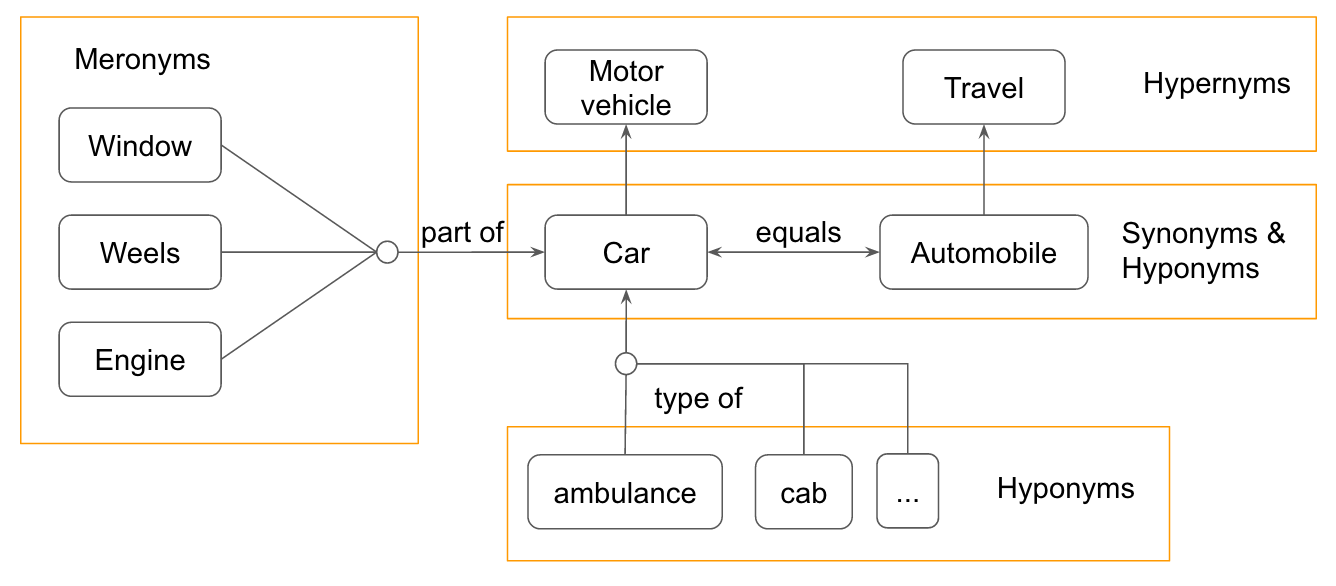
\includegraphics[width=0.7\textwidth]{wsd_analysis.png}
        \caption{"Semantic fields, hierarchies"}
        \label{wsd_analysis}
    \end{figure} 

  \emph{Meronyms} are ``part-of'' relations, \emph{hyponyms} have a ``type-of'' relation to a higher concept, called \emph{hypernyms}. In figure \ref{wsd_analysis} we see that from a single concept ``car'' we can infer a semantic field around it. We will see later how this works, a statistical concept around this is \emph{LSI} and \emph{probabilistic topic modelling}. The symbolic way is to use knowledge bases such as Wordnet or Wikipedia.\\

  In the text \emph{domain} of newspaper articles a few problems arise. Analyzing a long book, a long speech or journal articles from the scientific community, is easier compared to high varying fragments from different authors on different topics. A long book written by one person will use a specific language that is typical of that author. Speeches for a specific person contain similar concepts and often use the same language as well. In the scientific community rhethorial and anecdotal phrasing is uncommon. Facts, citation and correct formatting is of central importance. The text might be heterogenous but the fact remains that a certain wording / glossary, is shared throughout these examples.\\

  This does not hold true for newspaper articles. \emph{Topics} about different events co-occuring on the world. Different \emph{authors} with different writing styles. Different \emph{newspapers} with different directions of content presentation. \emph{Long} and very \emph{short} articles. And this does not take images, videos or comments into account. When dealing with a vast landscape of different topics, spanning connections between two documents becomes a hard task. In context of such sparse data, that is documents with almost no connecting words, clustering works poorly. This can also be described as a high variance problem, where each document contributes a lot of unseen words to the feature vector.\\

  In order to avoid these variance problems, we need to find a solution to \emph{WSD} and then apply a lifting from the original concept to a hypernym. Going back to figure \ref{wsd_analysis} we see that \emph{car} and \emph{motored vehicle} might mean the same thing. Both are about cars, if we project the concept \emph{car} to \emph{motored vehicle} the concept would connect both the documents containing car and motored vehicle. This is not always what we want to achieve but it could drastically improve similarity between documents that would miss each other by synonymy and polysemy.

\section{Selection}
\label{sec:selection}

  As described before we want to tackle \emph{WSD} and find ways to connect documents that share common meaning but not a lot of common words. To do so we have several strategies at our disposal. First, word pruning is presented, it is probably the most widely used technique for lowering dimensions and removing insignificant words. Second, synctactic parsing is described in by part of speech tagging, noun phrase extraction and named entity recognition. One topic which is left out are the kernels. They are important to retrieve better results in a semi supervised way but could not make it into the thesis experiments.

  \subsection{Word pruning}
  \label{sec:word_pruning}

    Before pruning words we have to convert the documents into a suitable vsm such as \emph{counting vectors} or \emph{TF-IDF} described in \ref{sec:bag_of_words}. The counting alone in its basic form is sufficient in telling if a term has a high or low connection with all other documents. The \emph{TF-IDF} on the other hand is a measure of importance and solely based on the resulting frequencey per word. It is possible to make significant pruning on both representations. The \emph{TF-IDF} variant is prefered as it normalizes frequencies. Higher or lower counts are weighted into a formula that better represents the significance of a term.\\

    Either way we need to create a cooccurence matrix $M = count(C, D)$ where $C$ is a corpus and $D$ is the dictionary of the corpus. Then we transform by \emph{TF-IDF}, $M = tfidf(M)$ or leave it with the \emph{term frequency}.\\

    Pruning $M$ is done by cutting off the documents with a very low ratio of counts with respect to all documents. This can be done by threshold in proportion to all terms, a percentage, removing $j$ terms. It can also be achieved by a hard count, cutting of all terms that have no counts higher than that. This means, we remove insignificant terms or terms that do not contribute to any connection. Semantically this means, we cut off words that have a high meaning in a single document and a very low in others. Those words are redundant, or in other words they have no discriminant value to the clustering process.

      \begin{equation}
      \begin{split}
        m &= [0, 1, 5, 0, 4, 0, 1, 1, 2, 3] \\
        m_s &= sort( [0, 0, 0, 1, 1, 1, 2, 3, 4, 5] ) \\
        percentcut(m_s, 0.2) &= [0, 1, 1, 1, 2, 3, 4, 5] \\
        totalcut(m_s, 1) &= [2, 3, 4, 5]
      \end{split}
      \end{equation}

    The min cut on percentage $0.2 = 20\%$ cuts the first 2 samples or removes the first 6 in case of a total count. The parameter has to be varied, depending on the outcome of a cost function. Further we can take off the top $j$ words as well by the same principle. The problem with the top words is, that they highly correlate with a lot of different documents, meaning a high correlation between a term and the corpus. Leaving them out erases a lot of connections, resulting in more discriminant features. This is what we want to achieve, finding the middle words, that are common in certain documents and uncommon in others. During clustering this will result in much more coherent clusters.

      \begin{equation}
      \begin{split}
        m &= [0, 1, 5, 0, 4, 0, 1, 1, 2, 3] \\
        m_s &= sort( [0, 0, 0, 1, 1, 1, 2, 3, 4, 5] ) \\
        maxcut(m_s, 0.8) &= [0, 0, 0, 1, 1, 1, 2, 3]
      \end{split}
      \end{equation}

    The max cut works with a ratio that selects from lowest to highest 80\% except the last 20\%. Note that the samples are not on $m$ dimensional vectors. For this to work we have to aggregate the counts and then prune the most insignificant words. The great thing of this approach is that it can follow any feature selection strategy. There are several ways to intialize the dictionary, which itself is a feature selection. By using this approach we can make sure that better feature selection strategies are fine tuned by upper and lower bounds.

  \subsection{Syntactic parsing}
  \label{sec:syntactic_parsing}

  Syntactic parsing reduces symbols or characters, to a parsed tree of following expressions. What the actual alphabet, in this sense valid characters of a language defines is defined within the specific domain. For this we often state grammars and valid tokens of an alphabet. This if often found for file standards like \emph{json}, \emph{csv} or \emph{programming languages}. When it comes to parsing expressions from English language to a meaningful representation for the computer, the problem statement gets a lot more difficult. It starts with defining what the actual valid words look like. Generally one could provide a dictionary as before. Everything not in the dictionary is not a valid character set. The problem becomes clear, because newspaper articles use different language styles and often make up words. However statistical parsers like the \emph{Stanford} parser are very accurate in identifying valid syntactic English expressions. In order to work, most of these parsers are supervised, trained models on a subset of English training samples. In the following we will look more closely at noun phrase extraction and named entity recognition. They can be used as initial seeds for the feature space of a corpus.

  \subsubsection{Noun phrases}

  bla

  \subsubsection{Named entities}

  bla


\section{External Knowledge}
\label{sec:semantic_selection}
  
  \newcommand\waw{\emph{Wordnet} and \emph{Wikipedia}}

  In order to enhance the syntactical selection models we can add a knowledge base such as \waw{}. The data reresentation is often defined as a typical dictionary. For a definition of a word we can infer semantic fields and additional text describing the words in more detail. Moreover knowledge bases such as \emph{Wikipedia} categorize/classify concepts into ontologies. \waw{} are great in the sense that human authors around the world add missing information and enhance the models frequently. The knoledge bases are enhanced frequently by writing rules and reviewing processes.

  \subsection{Wordnet}
  \label{sec:wordnet}

  \subsection{Wikipedia}
  \label{sec:wikpedia}
  

